\documentclass[10pt]{article}\usepackage[]{graphicx}\usepackage[]{color}
%% maxwidth is the original width if it is less than linewidth
%% otherwise use linewidth (to make sure the graphics do not exceed the margin)
\makeatletter
\def\maxwidth{ %
  \ifdim\Gin@nat@width>\linewidth
    \linewidth
  \else
    \Gin@nat@width
  \fi
}
\makeatother

\definecolor{fgcolor}{rgb}{0.345, 0.345, 0.345}
\newcommand{\hlnum}[1]{\textcolor[rgb]{0.686,0.059,0.569}{#1}}%
\newcommand{\hlstr}[1]{\textcolor[rgb]{0.192,0.494,0.8}{#1}}%
\newcommand{\hlcom}[1]{\textcolor[rgb]{0.678,0.584,0.686}{\textit{#1}}}%
\newcommand{\hlopt}[1]{\textcolor[rgb]{0,0,0}{#1}}%
\newcommand{\hlstd}[1]{\textcolor[rgb]{0.345,0.345,0.345}{#1}}%
\newcommand{\hlkwa}[1]{\textcolor[rgb]{0.161,0.373,0.58}{\textbf{#1}}}%
\newcommand{\hlkwb}[1]{\textcolor[rgb]{0.69,0.353,0.396}{#1}}%
\newcommand{\hlkwc}[1]{\textcolor[rgb]{0.333,0.667,0.333}{#1}}%
\newcommand{\hlkwd}[1]{\textcolor[rgb]{0.737,0.353,0.396}{\textbf{#1}}}%

\usepackage{framed}
\makeatletter
\newenvironment{kframe}{%
 \def\at@end@of@kframe{}%
 \ifinner\ifhmode%
  \def\at@end@of@kframe{\end{minipage}}%
  \begin{minipage}{\columnwidth}%
 \fi\fi%
 \def\FrameCommand##1{\hskip\@totalleftmargin \hskip-\fboxsep
 \colorbox{shadecolor}{##1}\hskip-\fboxsep
     % There is no \\@totalrightmargin, so:
     \hskip-\linewidth \hskip-\@totalleftmargin \hskip\columnwidth}%
 \MakeFramed {\advance\hsize-\width
   \@totalleftmargin\z@ \linewidth\hsize
   \@setminipage}}%
 {\par\unskip\endMakeFramed%
 \at@end@of@kframe}
\makeatother

\definecolor{shadecolor}{rgb}{.97, .97, .97}
\definecolor{messagecolor}{rgb}{0, 0, 0}
\definecolor{warningcolor}{rgb}{1, 0, 1}
\definecolor{errorcolor}{rgb}{1, 0, 0}
\newenvironment{knitrout}{}{} % an empty environment to be redefined in TeX

\usepackage{alltt}
% !Rnw weave = knitr
% sweave fig help:
% http://users.stat.umn.edu/~geyer/Sweave/foo.pdf
% borrowing design from roxygen -- AJB Jan 13

%% \VignetteIndexEntry{DFT benchmarks: fft vs FFT.}
%% \VignetteEngine{knitr}

\usepackage[T1]{fontenc}
\usepackage[utf8]{inputenc}
\usepackage{fancyvrb}
\usepackage[pdfborder={0 0 0}]{hyperref}
\usepackage{url}
\usepackage{upquote}
\usepackage{graphicx}
\usepackage{grffile}
\usepackage{amsmath}
\usepackage{amssymb}
\usepackage{float}
\usepackage{natbib}
\usepackage{geometry}
\geometry{verbose,tmargin=3cm,bmargin=5cm,lmargin=2.5cm,rmargin=2.5cm}
%\usepackage{fullpage}
%captions
\usepackage[font=sf, labelfont={sf,bf}, margin=2cm]{caption}
%
\usepackage{color}
%
%%
%% Mathematics definitions
%% do not use special characters!
%%
%TMP\newcommand{\dxx}[1]{\enm{#1}} %% null
\newcommand{\enm}[1]{\ensuremath{#1}} %% null
\newcommand{\dFT}[0]{\enm{\mathfrak{F}}} %% fourier transform operator (FT)
\newcommand{\dFTp}[1]{\enm{\dFT{}\{#1\}}} %% FT{...}
\newcommand{\df}[0]{\enm{x}} %% stationary signal f
\newcommand{\dF}[0]{\enm{X}} %% FT{f}
\newcommand{\dmod}[1]{\enm{\mathrm{mod} \{#1\}}}
\newcommand{\dmodF}[0]{\dmod{\Xfo_T{}}}
\newcommand{\dargF}[0]{\enm{\mathrm{arg} \{ \Xfo_T{} \}}}
\newcommand{\ds}[0]{\enm{s}} %% spectrum
\newcommand{\dS}[0]{\enm{S(f)}} %% Spectrum
\newcommand{\dsupsf}[1]{\enm{{}^{#1}\ds{}}} %% superscript spectrum front
\newcommand{\dsupSf}[1]{\enm{{}^{#1}\dS{}}} %% superscript Spectrum front
\newcommand{\dsupsb}[1]{\enm{\ds{}^{#1}}} %% superscript spectrum back
\newcommand{\dsupSb}[1]{\enm{\dS{}^{#1}}} %% superscript Spectrum back
\newcommand{\daF}[0]{\enm{| \Xfo_T |}} %% amplitude Spectrum
\newcommand{\daS}[0]{\enm{\sqrt{\Re^2 + \Im^2}}} %% amplitude Spectrum
\newcommand{\dpS}[0]{\enm{\tan^{-1}\left(\Im / \Re \right)}} %% phase Spectrum
\newcommand{\dESD}[0]{\enm{E(f)}} %\dsupSf{\mathrm{(E)}}} %% energy Spectral density
\newcommand{\dPSD}[0]{\dsupSf{\mathrm{(P)}}} %% power Spectral density
%%
\newcommand{\intone}{\enm{\int_{- \infty} ^{\infty}}}
\newcommand{\Fo}{\enm{\mathcal{F}}}
\newcommand{\Xfo}{\enm{\tilde{X}}}
\newcommand{\stochXfo}{\enm{\tilde{\mathcal{X}}}}
\newcommand{\rXfo}{\enm{\Xfo{}^R}}
\newcommand{\iXfo}{\enm{\Xfo{}^I}}
\newcommand{\Ex}{\enm{\mathcal{E}}}
\newcommand{\slfrac}[2]{\left.#1\middle/#2\right.}
\newcommand{\half}{\enm{\slfrac{1}{2}}}
\newcommand{\nhalf}{\enm{\slfrac{-1}{2}}}
\newcommand{\Var}{\enm{\mathcal{V}}}
\newcommand{\Cov}{\enm{\mathrm{Cov}}}
\newcommand{\conv}{\ensuremath{\ast}}
%%
\newcommand{\dACV}[1]{\enm{\mathcal{R}(#1)}}
\newcommand{\dX}[1]{\enm{\mathcal{X}(#1)}}
\newcommand{\dXsub}[1]{\enm{\mathcal{X}_{#1}}}
\newcommand{\dXstoch}[0]{\dX{t}}
\newcommand{\dXstochd}[0]{\dXsub{n}}
\newcommand{\dXlag}[0]{\dX{\tau}}
\newcommand{\dXrealiz}[0]{\enm{X_T(t)}}
%%

%%
\newcommand{\SC}[1]{\textsc{#1}}
\newcommand{\SCY}[0]{\SC{Yes}}
\newcommand{\SCN}[0]{\SC{No}}
\newcommand{\Rcmd}[1]{\texttt{#1}}
\newcommand{\psd}[0]{\href{http://abarbour.github.com/psd/}{\color{blue}\Rcmd{psd}}}
\newcommand{\naive}[0]{na\"{\i}ve}
\newcommand{\bidx}[1]{\index{#1}{\textbf{#1}}} 
\newcommand{\idx}[1]{\index{#1}{#1}} 
%% path, filename, caption, label
\newcommand{\listing}[4]{        %
  \begin{figure}[H]              %
    \centering                   %
    \VerbatimInput[numbers=left, %
      frame=single,              %
      label=#2]{#1}              %
    \caption{#3}                 %
    \label{#4}                   %
  \end{figure}                   %
}
\author{Andrew J. Barbour}
\title{Benchmarks for Discrete Fourier Transforms in R}
\IfFileExists{upquote.sty}{\usepackage{upquote}}{}
\begin{document}
\maketitle
\begin{abstract}
The base DFT calculator in R, \Rcmd{stats::fft}, uses
the Mixed-Radix algorithm of \citet{singleton1969}.
In this vignette we show how 
this calculator compares
to \Rcmd{FFT} in the \Rcmd{fftw} package \citep{fftw}, which uses the
FFTW algorithm of \citet{frigo2005}.
For univariate DFT computations,
the methods are nearly equivalent with two exceptions which
are not mutually exclusive: 
(A) the series to be transformed is very long, and 
especially (B) when the series length is not highly composite.
In both exceptions the algorithm \Rcmd{FFT} outperforms \Rcmd{fft}.
\end{abstract}
\tableofcontents
\section{Benchmarking function}
We use both functions in their default state, and ask them
to transform the same univariate random series.
Benchmark information comes from the \Rcmd{rbenchmark}
program, and the versatile \Rcmd{plyr} and
\Rcmd{reshape2} packages are used to manipulate the information
for this presentation; \Rcmd{ggplot2} is used for plotting. 
First we load the libraries needed:
\begin{knitrout}
\definecolor{shadecolor}{rgb}{0.969, 0.969, 0.969}\color{fgcolor}\begin{kframe}
\begin{alltt}
\hlkwd{rm}\hlstd{(}\hlkwc{list}\hlstd{=}\hlkwd{ls}\hlstd{())}
\hlkwd{library}\hlstd{(fftw)}
\hlkwd{library}\hlstd{(rbenchmark)}
\hlkwd{library}\hlstd{(plyr)}
\hlkwd{library}\hlstd{(reshape2)}
\hlkwd{library}\hlstd{(ggplot2)}
\end{alltt}
\end{kframe}
\end{knitrout}
and create a benchmark function:
\begin{knitrout}
\definecolor{shadecolor}{rgb}{0.969, 0.969, 0.969}\color{fgcolor}\begin{kframe}
\begin{alltt}
\hlstd{reps} \hlkwb{<-} \hlnum{10}
\hlstd{dftbm} \hlkwb{<-} \hlkwa{function}\hlstd{(}\hlkwc{nd}\hlstd{,} \hlkwc{repls}\hlstd{=reps)\{}
        \hlkwd{set.seed}\hlstd{(}\hlnum{1234}\hlstd{)}
        \hlstd{x} \hlkwb{<-} \hlkwd{rnorm}\hlstd{(nd,} \hlkwc{mean}\hlstd{=}\hlnum{0}\hlstd{,} \hlkwc{sd}\hlstd{=}\hlnum{1}\hlstd{)}
        \hlstd{bmd} \hlkwb{<-} \hlkwd{benchmark}\hlstd{(}\hlkwc{replications}\hlstd{=repls, fftw}\hlopt{::}\hlkwd{FFT}\hlstd{(x), stats}\hlopt{::}\hlkwd{fft}\hlstd{(x))}
        \hlstd{bmd}\hlopt{$}\hlstd{num_dat} \hlkwb{<-} \hlstd{nd}
        \hlstd{bmd}\hlopt{$}\hlstd{relative[}\hlkwd{is.na}\hlstd{(bmd}\hlopt{$}\hlstd{relative)]} \hlkwb{<-} \hlnum{1}   \hlcom{# NA happens.}
        \hlkwd{return}\hlstd{(bmd)}
\hlstd{\}}
\end{alltt}
\end{kframe}
\end{knitrout}

\section{Highly composite (HC) series}
It's well known that DFT algorithms are most efficient
for ``Highly Composite Numbers"\footnote{
This is the reason for the \Rcmd{stats::nextn} function.
}, specifically multiples of (2,3,5).

So, we create a vector of series lengths we wish to benchmark
\begin{knitrout}
\definecolor{shadecolor}{rgb}{0.969, 0.969, 0.969}\color{fgcolor}\begin{kframe}
\begin{alltt}
\hlstd{(nterms.even} \hlkwb{<-} \hlkwd{round}\hlstd{(}\hlnum{2}\hlopt{**}\hlkwd{seq.int}\hlstd{(}\hlkwc{from}\hlstd{=}\hlnum{4}\hlstd{,}\hlkwc{to}\hlstd{=}\hlnum{20}\hlstd{,}\hlkwc{by}\hlstd{=}\hlnum{1}\hlstd{)))}
\end{alltt}
\begin{verbatim}
##  [1]      16      32      64     128     256     512    1024    2048
##  [9]    4096    8192   16384   32768   65536  131072  262144  524288
## [17] 1048576
\end{verbatim}
\end{kframe}
\end{knitrout}
and use it with \Rcmd{lapply} and the benchmark function
previously defined.
These data are further distilled into a usable format
with \Rcmd{ldply}:
\begin{knitrout}
\definecolor{shadecolor}{rgb}{0.969, 0.969, 0.969}\color{fgcolor}\begin{kframe}
\begin{alltt}
\hlstd{bench.even} \hlkwb{<-} \hlkwa{function}\hlstd{()\{}
  \hlstd{benchdat.e} \hlkwb{<-} \hlstd{plyr}\hlopt{::}\hlkwd{ldply}\hlstd{(}\hlkwd{lapply}\hlstd{(}\hlkwc{X}\hlstd{=nterms.even,} \hlkwc{FUN}\hlstd{=dftbm))}
  \hlstd{\}}
\hlkwd{bench.even}\hlstd{()}
\end{alltt}
\end{kframe}
\end{knitrout}

\section{Non highly composite (NHC) series}
DFT algorithms can have drastically reduced performance
if the series length is not highly composite (NHC).
We now test NHC series by adding one to the HC series-length
vector (also restricting the total length for sanity's sake):
\begin{knitrout}
\definecolor{shadecolor}{rgb}{0.969, 0.969, 0.969}\color{fgcolor}\begin{kframe}
\begin{alltt}
\hlstd{nterms.odd} \hlkwb{<-} \hlstd{nterms.even} \hlopt{+} \hlnum{1}
\hlstd{nterms.odd} \hlkwb{<-} \hlstd{nterms.odd[nterms.odd} \hlopt{<} \hlnum{50e3}\hlstd{]} \hlcom{# painfully long otherwise!}
\end{alltt}
\end{kframe}
\end{knitrout}
and performing the full set of benchmarks again:
\begin{knitrout}
\definecolor{shadecolor}{rgb}{0.969, 0.969, 0.969}\color{fgcolor}\begin{kframe}
\begin{alltt}
\hlstd{bench.odd} \hlkwb{<-} \hlkwa{function}\hlstd{()\{}
  \hlstd{benchdat.o} \hlkwb{<-} \hlstd{plyr}\hlopt{::}\hlkwd{ldply}\hlstd{(}\hlkwd{lapply}\hlstd{(}\hlkwc{X}\hlstd{=nterms.odd,} \hlkwc{FUN}\hlstd{=dftbm))}
  \hlstd{\}}
\hlkwd{bench.odd}\hlstd{()} \hlcom{# FAIR WARNING: this can take a while!!}
\end{alltt}
\end{kframe}
\end{knitrout}

\section{Visualization}
In order to plot the results, we need to 
perform some map/reduce operations on the data
\citep{wickham2010}. We intend to show faceted \Rcmd{ggplot2}-based
figures with row-wise summary information\footnote{
Based on this post:\\
{\small
\url{http://geokook.wordpress.com/2012/12/29/row-wise-summary-curves-in-faceted-ggplot2-figures/}
}
} so we can easily intercompare the benchmark data.
The benchmark data we will show
are \Rcmd{user.self}, \Rcmd{sys.self}, \Rcmd{elapsed}, and \Rcmd{relative}.
The results are shown
in Figure \ref{fig:results}.

\begin{knitrout}
\definecolor{shadecolor}{rgb}{0.969, 0.969, 0.969}\color{fgcolor}\begin{kframe}
\begin{alltt}
\hlstd{pltbench} \hlkwb{<-} \hlkwa{function}\hlstd{(}\hlkwc{lentyp}\hlstd{=}\hlkwd{c}\hlstd{(}\hlstr{"even"}\hlstd{,}\hlstr{"odd"}\hlstd{))\{}
  \hlstd{benchdat} \hlkwb{<-} \hlkwd{switch}\hlstd{(}\hlkwd{match.arg}\hlstd{(lentyp),} \hlkwc{even}\hlstd{=benchdat.e,} \hlkwc{odd}\hlstd{=benchdat.o)}
  \hlkwd{stopifnot}\hlstd{(}\hlkwd{exists}\hlstd{(}\hlstr{"benchdat"}\hlstd{))}
  \hlstd{tests} \hlkwb{<-} \hlkwd{unique}\hlstd{(benchdat}\hlopt{$}\hlstd{test)}
  \hlcom{## subset only information we care about}
  \hlstd{allbench.df.drp} \hlkwb{<-} \hlkwd{subset}\hlstd{(benchdat,}
        \hlkwc{select}\hlstd{=}\hlkwd{c}\hlstd{(test, num_dat, user.self, sys.self, elapsed, relative))}
  \hlcom{## reduce data.frame with melt}
  \hlstd{allbench.df.mlt} \hlkwb{<-} \hlstd{reshape2}\hlopt{::}\hlkwd{melt}\hlstd{(allbench.df.drp,}
                                    \hlkwc{id.vars}\hlstd{=}\hlkwd{c}\hlstd{(}\hlstr{"test"}\hlstd{,}\hlstr{"num_dat"}\hlstd{))}
  \hlcom{## calculate the summary information to be plotted:}
  \hlstd{tmpd} \hlkwb{<-} \hlstd{plyr}\hlopt{::}\hlkwd{ddply}\hlstd{(allbench.df.mlt,}
                      \hlkwd{.}\hlstd{(variable,  num_dat),}
                      \hlstd{summarise,}
                      \hlkwc{summary}\hlstd{=}\hlstr{"medians"}\hlstd{,}
                      \hlkwc{value}\hlstd{=ggplot2}\hlopt{::}\hlkwd{mean_cl_normal}\hlstd{(value)[}\hlnum{1}\hlstd{,}\hlnum{1}\hlstd{])}
  \hlcom{## create copies for each test and map to data.frame}
  \hlstd{allmeds} \hlkwb{<<-} \hlstd{plyr}\hlopt{::}\hlkwd{ldply}\hlstd{(}\hlkwd{lapply}\hlstd{(}\hlkwc{X}\hlstd{=tests,}
                                 \hlkwc{FUN}\hlstd{=}\hlkwa{function}\hlstd{(}\hlkwc{x}\hlstd{,}\hlkwc{df}\hlstd{=tmpd)\{}
                                       \hlstd{df}\hlopt{$}\hlstd{test} \hlkwb{<-} \hlstd{x;} \hlkwd{return}\hlstd{(df)}
                                     \hlstd{\}))}
  \hlcom{## plot the benchmark data}
  \hlcom{# 1/sqrt(n) standard errors [assumes N(0,1)]}
  \hlstd{g} \hlkwb{<-} \hlkwd{ggplot}\hlstd{(}\hlkwc{data}\hlstd{=allbench.df.mlt,}
              \hlkwd{aes}\hlstd{(}\hlkwc{x}\hlstd{=}\hlkwd{log10}\hlstd{(num_dat),}
                  \hlkwc{y}\hlstd{=}\hlkwd{log2}\hlstd{(value),}
                  \hlkwc{ymin}\hlstd{=}\hlkwd{log2}\hlstd{(value}\hlopt{*}\hlstd{(}\hlnum{1}\hlopt{-}\hlnum{1}\hlopt{/}\hlkwd{sqrt}\hlstd{(reps))),}
                  \hlkwc{ymax}\hlstd{=}\hlkwd{log2}\hlstd{(value}\hlopt{*}\hlstd{(}\hlnum{1}\hlopt{+}\hlnum{1}\hlopt{/}\hlkwd{sqrt}\hlstd{(reps))),}
                  \hlkwc{colour}\hlstd{=test,}
                  \hlkwc{group}\hlstd{=test))} \hlopt{+}
       \hlkwd{scale_colour_discrete}\hlstd{(}\hlkwc{guide}\hlstd{=}\hlstr{"none"}\hlstd{)} \hlopt{+}
       \hlkwd{theme_bw}\hlstd{()}\hlopt{+}
       \hlkwd{ggtitle}\hlstd{(}\hlkwd{sprintf}\hlstd{(}\hlstr{"DFT benchmarks of %s length series"}\hlstd{,}\hlkwd{toupper}\hlstd{(lentyp)))} \hlopt{+}
       \hlkwd{ylim}\hlstd{(}\hlkwd{c}\hlstd{(}\hlopt{-}\hlnum{11}\hlstd{,}\hlnum{11}\hlstd{))}\hlopt{+}
       \hlkwd{xlim}\hlstd{(}\hlkwd{c}\hlstd{(}\hlnum{0.5}\hlstd{,}\hlnum{6.5}\hlstd{))}

  \hlcom{## add previous summary curves if exist}
  \hlkwa{if} \hlstd{(}\hlkwd{exists}\hlstd{(}\hlstr{"allmeds.prev"}\hlstd{))\{}
     \hlstd{g} \hlkwb{<-} \hlstd{g} \hlopt{+} \hlkwd{geom_path}\hlstd{(}\hlkwc{size}\hlstd{=}\hlnum{1.5}\hlstd{,} \hlkwc{colour}\hlstd{=}\hlstr{"dark grey"}\hlstd{,} \hlkwc{data}\hlstd{=allmeds.prev,}
                        \hlkwd{aes}\hlstd{(}\hlkwc{group}\hlstd{=test))}
                        \hlstd{\}}
  \hlcom{## create a facetted version}
  \hlstd{g2} \hlkwb{<-} \hlstd{g} \hlopt{+} \hlkwd{facet_grid}\hlstd{(variable}\hlopt{~}\hlstd{test)} \hlcom{#, scales="free_y")}
  \hlcom{## add the summary data as a line}
  \hlstd{g3} \hlkwb{<-} \hlstd{g2} \hlopt{+} \hlkwd{geom_path}\hlstd{(}\hlkwc{colour}\hlstd{=}\hlstr{"black"}\hlstd{,} \hlkwc{data}\hlstd{=allmeds,} \hlkwd{aes}\hlstd{(}\hlkwc{group}\hlstd{=test))}
  \hlcom{## and finally the data}
  \hlkwd{print}\hlstd{(g4} \hlkwb{<<-} \hlstd{g3} \hlopt{+} \hlkwd{geom_pointrange}\hlstd{())}
\hlstd{\}}
\end{alltt}
\end{kframe}
\end{knitrout}

\begin{knitrout}
\definecolor{shadecolor}{rgb}{0.969, 0.969, 0.969}\color{fgcolor}\begin{kframe}
\begin{alltt}
\hlkwd{pltbench}\hlstd{(}\hlstr{"even"}\hlstd{)}
\hlstd{allmeds.prev} \hlkwb{<-} \hlstd{allmeds}
\hlkwd{pltbench}\hlstd{(}\hlstr{"odd"}\hlstd{)}
\end{alltt}
\end{kframe}
\end{knitrout}

\begin{figure}[htb!]
\begin{center}
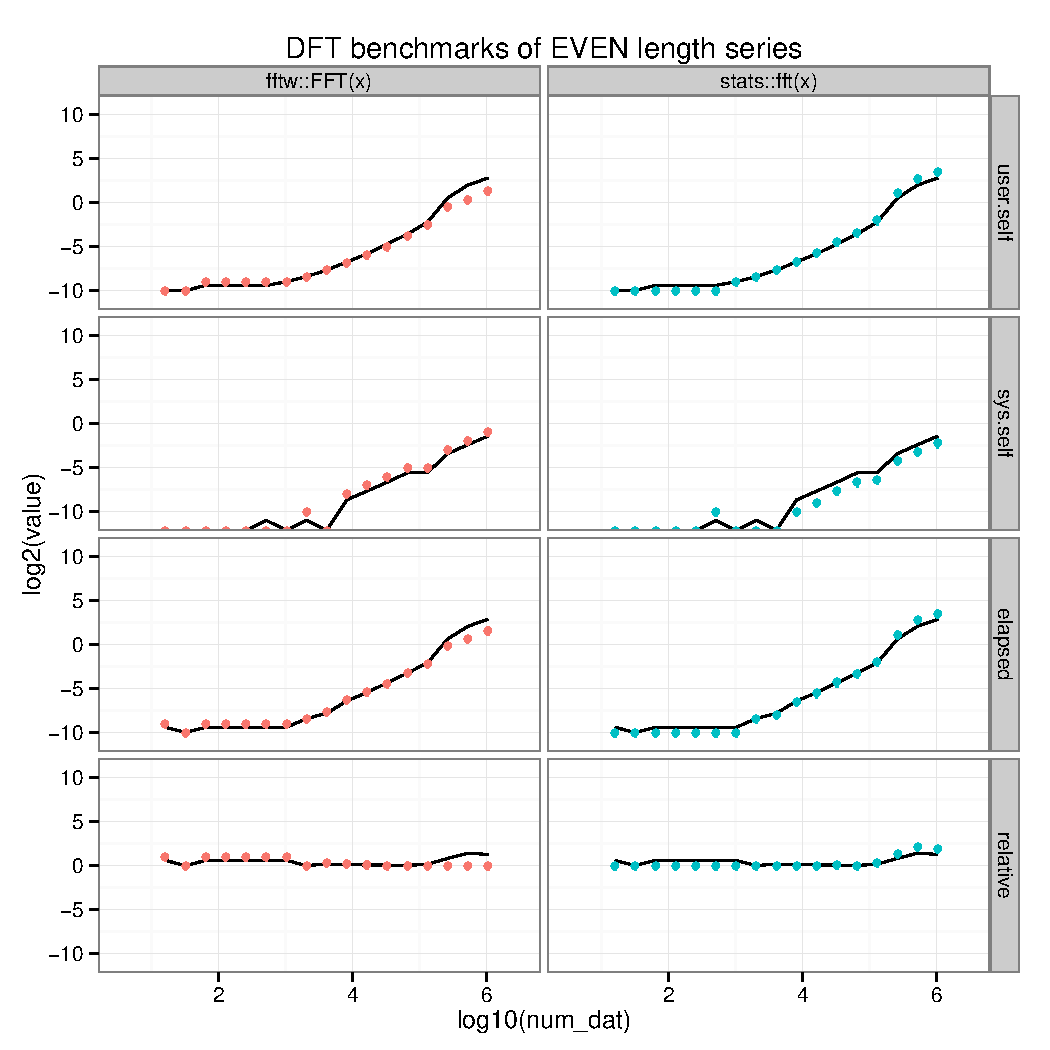
\includegraphics[width=0.5\textwidth]{fftw_bench_even}%
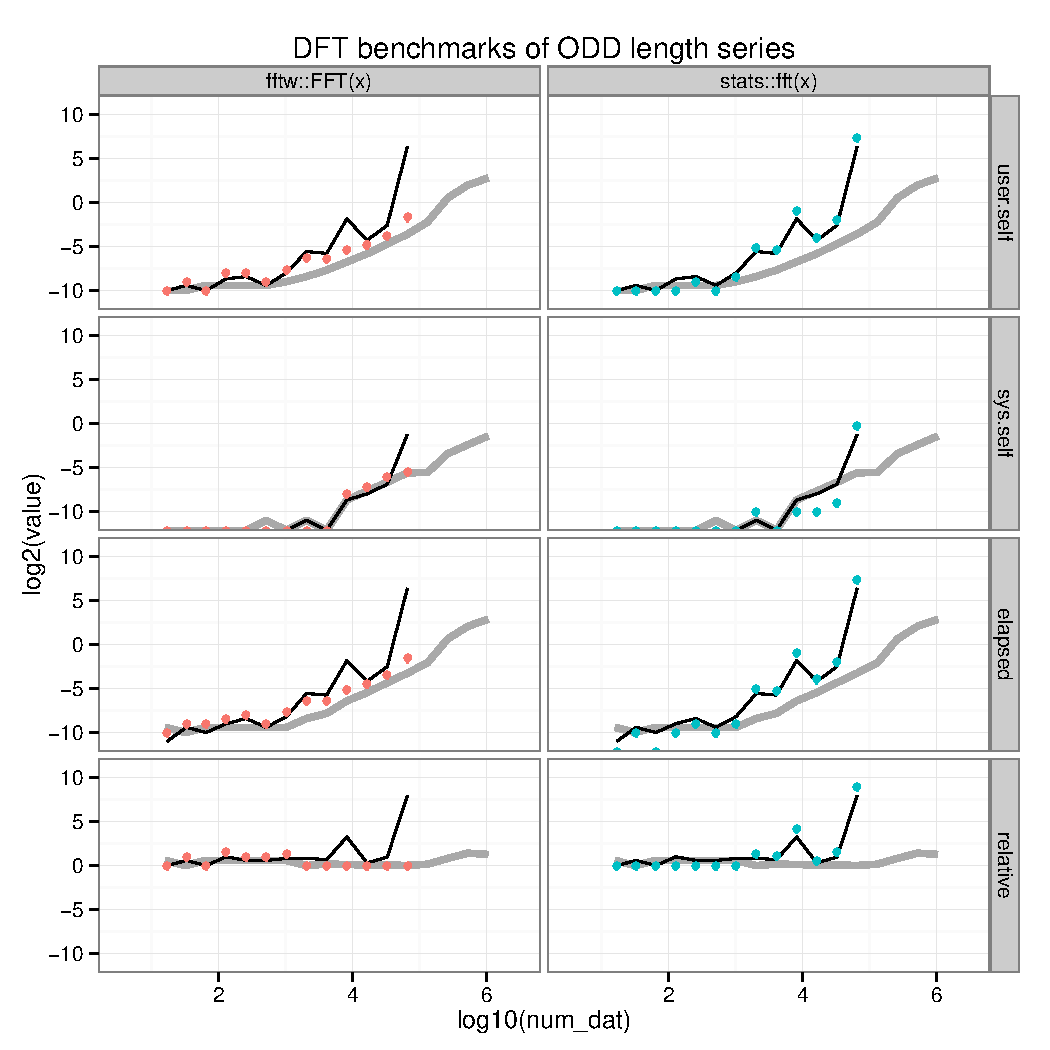
\includegraphics[width=0.5\textwidth]{fftw_bench_odd}
\caption{ DFT benchmark results for HC series lengths (left),
and NHC series lengths (right) as a function of logarithmic
series length.  In each figure, the left
facet-column is for results from \Rcmd{fftw::FFT} and the right
column is for \Rcmd{stats::fft}.
We also show the summary curves from the HC results
in the NHC frames (thick grey curve)
to highlight the drastic degradation in performance.}
\label{fig:results}
\end{center}
\end{figure}

\section{Conclusion}

Figure \ref{fig:results} compares the DFT
calculations for HC and NHC length series.
For univariate DFT computations,
the methods are nearly equivalent with two exceptions which
are not mutually exclusive: 
(A) the series to be transformed is very long, and 
especially (B) when the series length is not highly composite.
In both exceptions the algorithm \Rcmd{FFT} outperforms \Rcmd{fft}.
In the case of exception (B), both methods have
drastically increased computation times; hence, zero padding should be
done to ensure the length does not adversely
affect the efficiency of the DFT calculator.

%\pagebreak

\section*{Session Info}
\begin{knitrout}
\definecolor{shadecolor}{rgb}{0.969, 0.969, 0.969}\color{fgcolor}\begin{kframe}
\begin{alltt}
\hlstd{utils}\hlopt{::}\hlkwd{sessionInfo}\hlstd{()}
\end{alltt}
\begin{verbatim}
## R version 3.1.2 (2014-10-31)
## Platform: x86_64-apple-darwin13.4.0 (64-bit)
## 
## locale:
## [1] en_US.UTF-8/en_US.UTF-8/en_US.UTF-8/C/en_US.UTF-8/en_US.UTF-8
## 
## attached base packages:
## [1] stats     graphics  grDevices utils     datasets  methods   base     
## 
## other attached packages:
## [1] knitr_1.9
## 
## loaded via a namespace (and not attached):
## [1] evaluate_0.5.5 formatR_1.0    highr_0.4      stringr_0.6.2 
## [5] tools_3.1.2
\end{verbatim}
\end{kframe}
\end{knitrout}

%% bib and index
\bibliographystyle{apalike}
\bibliography{REFS}

\end{document}
